\documentclass{beamer}
\usepackage{beamerthemesplit}
\usepackage{tikz}
\newcommand{\ds}{\displaystyle}
\newcommand{\eps}{\epsilon}
\newcommand{\wh}{\widehat}
\newcommand{\alp}{\alpha}
\newcommand{\bet}{\beta}
\newcommand{\gam}{\gamma}
\newcommand{\veps}{\varepsilon}
\newcommand{\etal}{\textit{et al.}~}
\newcommand{\xmu}{\mbox{\boldmath$\mu$}}
\newcommand{\xtheta}{\mbox{\boldmath$\theta$}}
\newcommand{\xxi}{\mbox{\boldmath$\xi$}}
\newcommand{\xSigma}{\mbox{\boldmath$\Sigma$}}
\newcommand{\sigr}{\sigma^2_r}
\newcommand{\tdel}{\tilde\Delta}
\newcommand{\bmsy}{B_{\rm msy}}
\newcommand{\cmsy}{C_{\rm msy}}
\newcommand{\hmsy}{H_{\rm msy}}
\newcommand{\lsp}{\!\,}
\newcommand{\vphi}{\varphi}
\newcommand{\vs}{\textit{vs.}~}
\newcommand{\eg}{\textit{eg.}~}

\usetheme{Madrid}
\usecolortheme{dolphin}
\title{Conditioning IOTC Albacore OMs using the ABC approach}
\author{R. Hillary \& I. Mosqueira}
\institute{CSIRO Environment (AU) \& Wageningen Marine Research (NL)}
\titlegraphic{
    
\includegraphics[width=2cm,height=2cm]{CSIRO.png}\hspace{1cm}
\includegraphics[width=3cm,height=2cm]{UWag.png}
}

\begin{document}
\maketitle

% frame 1
\begin{frame}
\frametitle{Outline}
\begin{itemize}
    \item Presentation of paper \textit{IOTC--2024--WPM15--08}
    \item Conditioning of ALB OMs using ABC MCMC approach:
        \vspace{0.25cm} 
        \begin{enumerate}
            \item Model structure(s) \& time-line
            \item Input data
            \item Stock status prior scenarios
            \item Axes of uncertainty
            \item Results
            \item Next steps
        \end{enumerate}
\end{itemize}
\end{frame}

% frame 2
\begin{frame}
\frametitle{OM model structure: population dynamics}
\begin{itemize}
    \item Timeline: 2000 to 2020 (covers all existing cohorts)
    \item Age, sex and quarterly structured population model
    \item Beverton-Holt with exploited equilibrium initialisation
    \item Designed to mimic current assessment model structure
    \item Reproduces all key stock status variables:
        \vspace{0.25cm}
        \begin{enumerate}
            \item MSY variables: $\bmsy$, $\hmsy$, \& $\cmsy$
            \item Relative biomass (\eg relative to $B_0$)
        \end{enumerate}
\end{itemize}
\end{frame}

% frame 3
\begin{frame}
\frametitle{OM model structure: fishery dynamics}
\begin{itemize}
    \item Merge ``common'' seasonal LL fleets 1--4
    \item Retain single PS and ``Other'' fleet: 6 in total
    \item Size data from LL and PS data (aggregated across time)
    \item LL CPUE from a given fleet (not jointly at this time)
    \item Seasonal \vs annual catchability explored
\end{itemize}
\end{frame}

% frame 4
\begin{frame}
\frametitle{Stock status prior information}
\begin{itemize}
    \item Key feature of ABC approach
    \item Impose status priors (\eg from assessment) on OM
    \item Explore 4 types:
        \vspace{0.25cm}
        \begin{enumerate}
            \item Relative SSB: prior mean/SD for any range of years
            \item $\bmsy$ ratio: prior mean/SD for any range of years
            \item $\hmsy$ ratio: prior mean/SD for any range of years
            \item Overfishing probability: penalise \emph{only if} $H>\hmsy$
        \end{enumerate}
        \vspace{0.25cm}
    \item Integrate status information with LF \& CPUE data
    \item Here is where it diverges from assessment-to-OM approach
\end{itemize}
\end{frame}

% frame 5
\begin{frame}
\frametitle{Suite of stock status priors}
\begin{itemize}
    \item Relative SSB: year 2000 mean (CI) of 0.5 (0.3--0.7)
    \item $\bmsy$ ratio: 2019, 2020 mean 2.25, 2 with SD 0.35
    \item $\hmsy$ ratio: 2000, 2020 mean of 0.6 with SD 0.2
    \item Overfishing penalty: $\mathbb{P}\left(H/\hmsy>2\right)\leq 0.05$ 
    \item This removes small numbers of runs with very high $H$
\end{itemize}
\end{frame}

% frame 6
\begin{frame}
\frametitle{Covering previous axes of uncertainty}
\begin{enumerate}
    \item Steepness \& $M$: covariance joint prior (not discrete grid)
    \item $\sigr$: (i) fixed at 0.3; (ii) estimated with prior CI 0.2--0.5  
    \item LF: weight/influence (aggregating and ABC discrepancy) 
    \item LL catchability: alternative 1\% annual increasing trend
    \item CPUE series: seasonal $q$ using fleet 1 and 3 \emph{separately}
\end{enumerate}
\end{frame}

% frame 8
\begin{frame}
\frametitle{OM conditioning scenarios}
\begin{itemize}
  \item Explored seven individual scenarios for conditioning:
  \vspace{0.25cm}
  \begin{enumerate}
      \item \textbf{R1}: CPUE fleet 1, SSB but \emph{not} $\hmsy$ priors
      \item \textbf{R1a}: CPUE fleet 3, SSB \emph{and} $\hmsy$ priors 
      \item \textbf{R1b}: same as \textbf{R1} with additional overfishing penalty
      \item \textbf{R2}: same as \textbf{R1} but $\sigr$ estimated
      \item \textbf{R2a}: same as \textbf{R1a} but $\sigr$ estimated 
      \item \textbf{R2b}: same as \textbf{R1b} but $\sigr$ estimated 
      \item \textbf{R3}: same as \textbf{R1} with 1\% \textit{p.a.} $\uparrow$ $q$ trend
      \item \textbf{R3a}: same as \textbf{R1a} with 1\% \textit{p.a.} $\uparrow$ $q$ trend
  \end{enumerate}
\end{itemize}
\end{frame}

% frame 9
\begin{frame}
    \frametitle{Approximate Bayesian Computation (ABC)}
\begin{itemize}
    \item Relaxes idea of strict likelihood: $\ell(D\,|\,\xtheta)$
    \item Focus is on derived quantities: $X=f(\xtheta)$
    \item Instead define a discrepancy function: $\pi(D,X)$
    \item Prior $\pi(\xtheta)$ has a wider role in ABC format
    \item Now includes stock status prior information
    \item Approximate posterior defined as follows:
        \begin{equation*}
            \ds \tilde\pi(\xtheta\,|\,D)\propto \pi(D,X)\pi(\xtheta)
        \end{equation*}
    \item Custom MCMC algorithm to sample from $\tilde\pi(\xtheta\,|\,D)$
\end{itemize}
\end{frame}

% frame 10
\begin{frame}
    \frametitle{Discrepancy function \& priors}
\begin{itemize}
    \item Deconstructing the discrepancy function, $\pi(D,X)$
    \item Data elements:
        \vspace{0.2cm}
        \begin{enumerate}
            \item CPUE: single fleet quarterly biomass index
            \item LF: time-averaged Kullback-Leibler divergence 
        \end{enumerate}
        \vspace{0.2cm}
    \item Parameter and process variable prior, $\pi(\xtheta)$:
        \vspace{0.2cm} 
        \begin{enumerate}
            \item Direct parameter prior quasi-uninformative
            \item Implied prior on $\xtheta$ via stock status priors
            \item Informative prior on $\sigr$ (inverse-gamma)
        \end{enumerate} 
\end{itemize}
\end{frame}

% frame 11
\begin{frame}
    \frametitle{Fits to data: CPUE indices}
\begin{itemize}
    \item Fleet 1 (\textbf{R1}, left) \& fleet 3 (\textbf{R1a}, right):
\end{itemize}
\vspace{0.25cm}
\begin{figure}
\begin{center}
        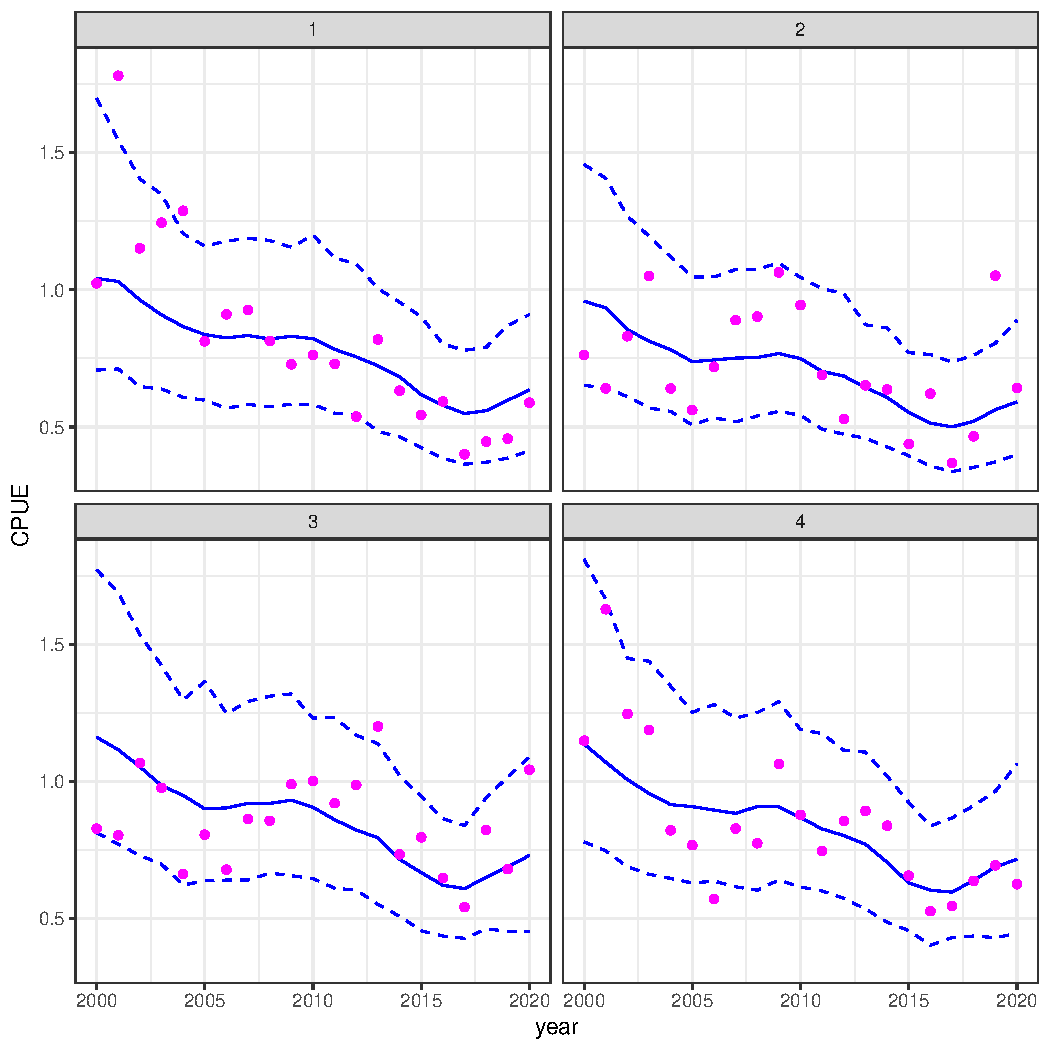
\includegraphics[width=6cm,height=6cm]{figs/case4_cpuefits.pdf}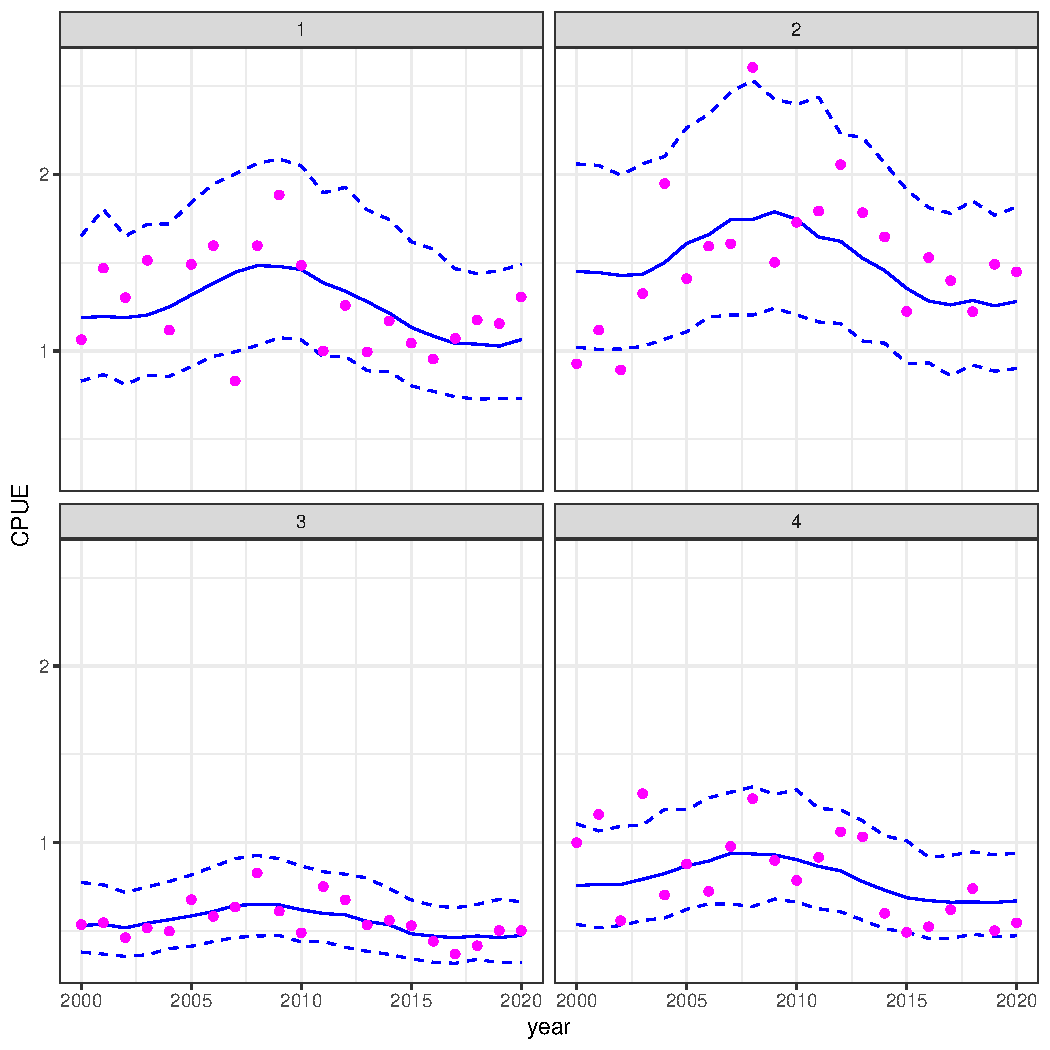
\includegraphics[width=6cm,height=6cm]{figs/case4a_cpuefits.pdf}
    \end{center}
\end{figure}
\end{frame}
% frame 12
\begin{frame}
    \frametitle{Fits to data: Length frequency data}
\begin{itemize}
    \item Scenario \textbf{R1} (left) \& \textbf{R1a} (right):
\end{itemize}
\vspace{0.25cm}
\begin{figure}
\begin{center}
        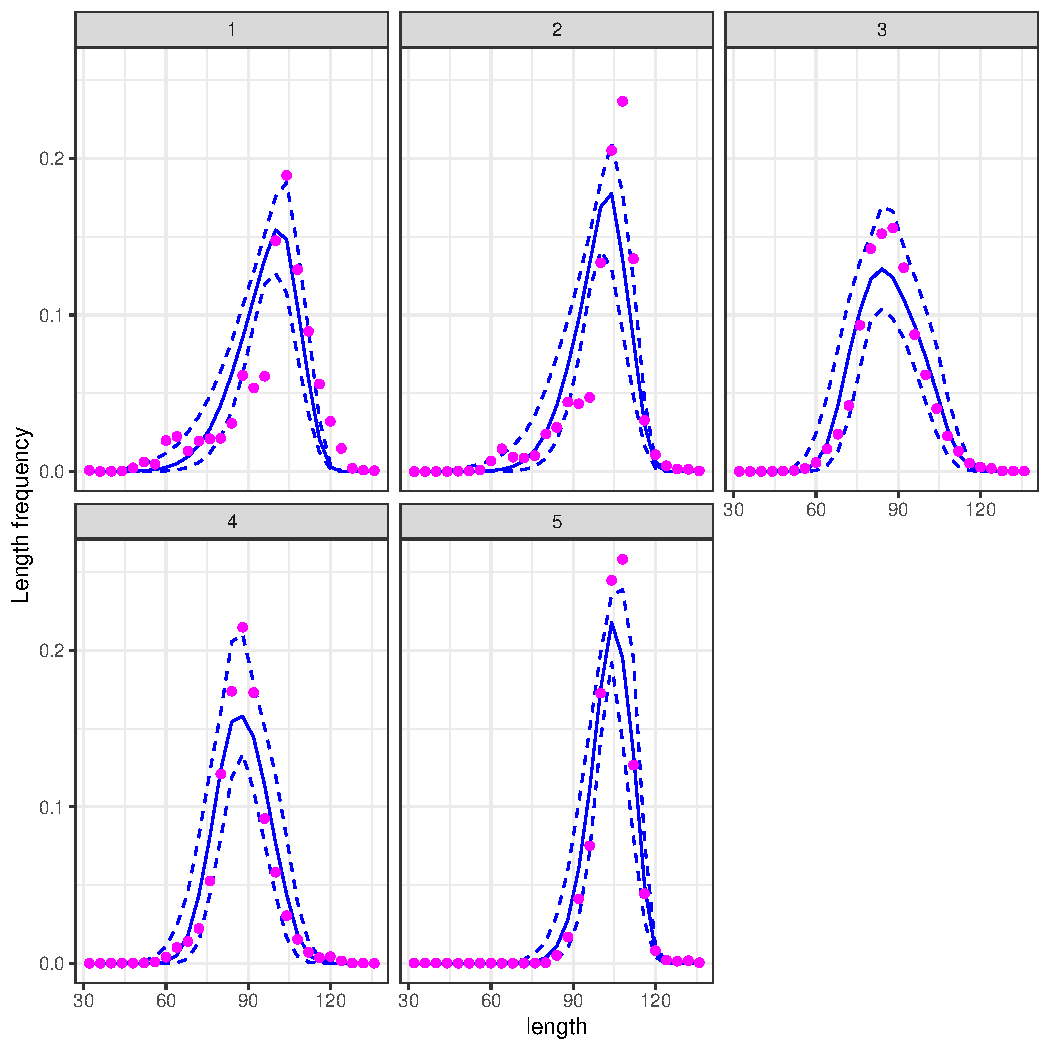
\includegraphics[width=6cm,height=6cm]{figs/case4_lffits.pdf}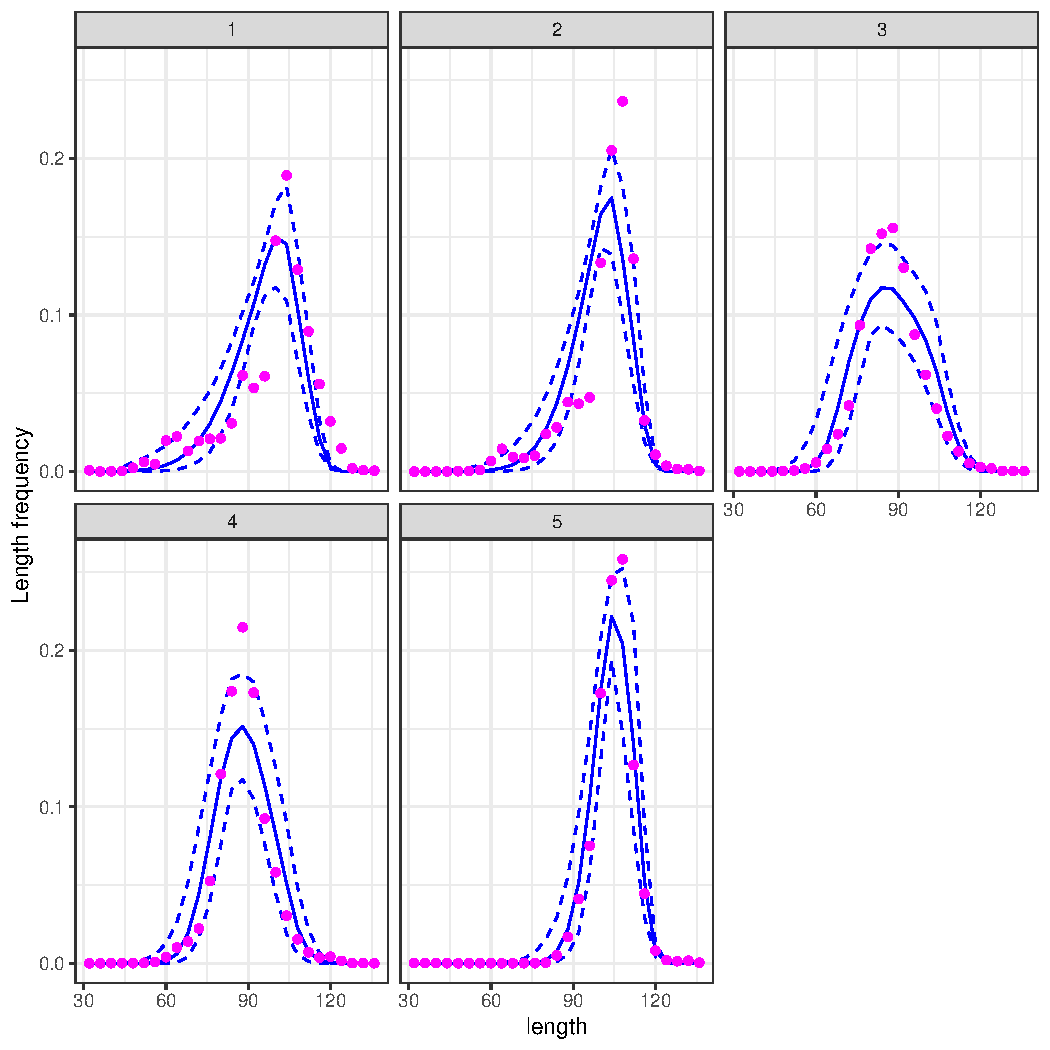
\includegraphics[width=6cm,height=6cm]{figs/case4a_lffits.pdf}
    \end{center}
\end{figure}
\end{frame}
% frame 13
\begin{frame}
    \frametitle{Population dynamics}
\begin{itemize}
    \item Scenario \textbf{R1} (top) \& \textbf{R1a} (bottom):
    \item SSB depletion (l), $\bmsy$ ratio (m), recruitment (r)
\end{itemize}
\begin{figure}
\begin{center}
       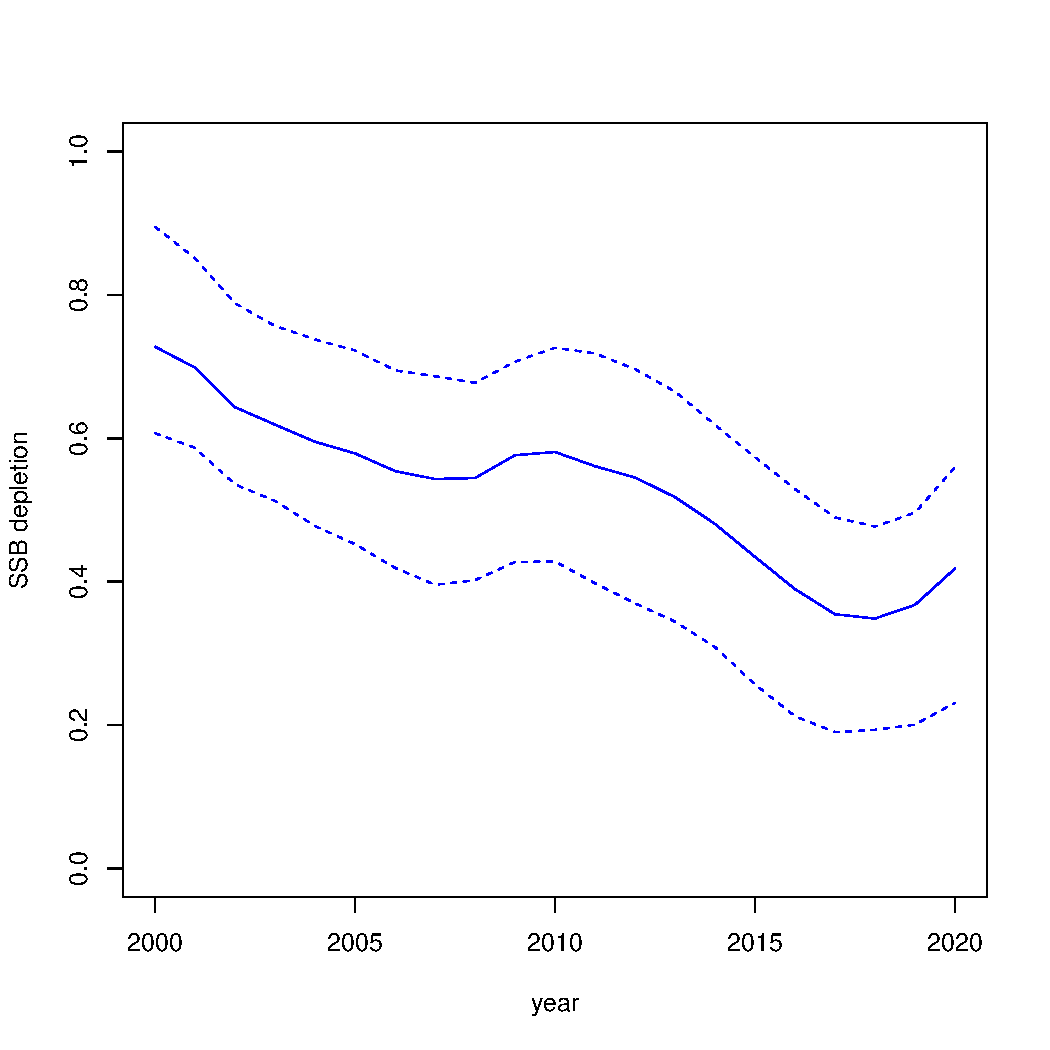
\includegraphics[width=3.5cm,height=3.5cm]{figs/case4_dep.pdf} 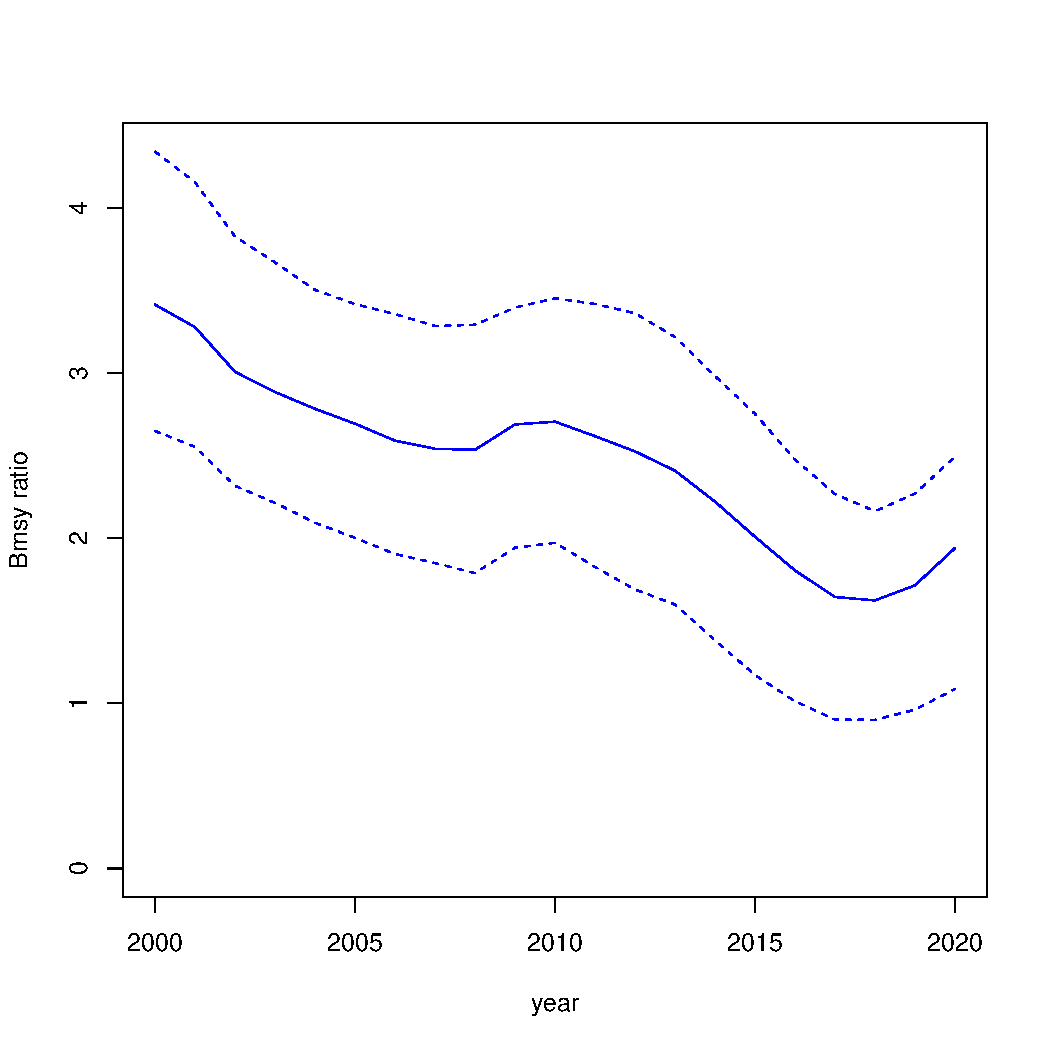
\includegraphics[width=3.5cm,height=3.5cm]{figs/case4_bmsy.pdf}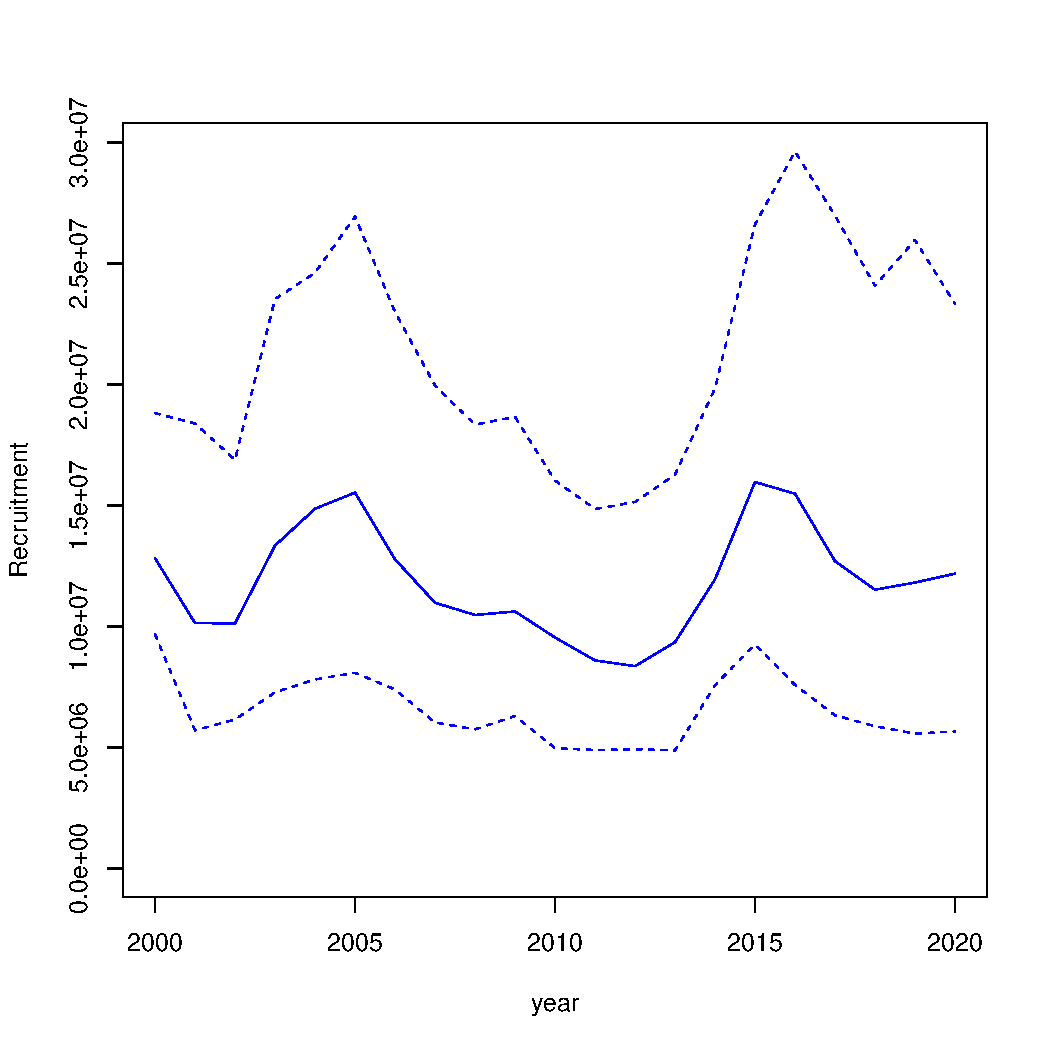
\includegraphics[width=3.5cm,height=3.5cm]{figs/case4_rec.pdf}
        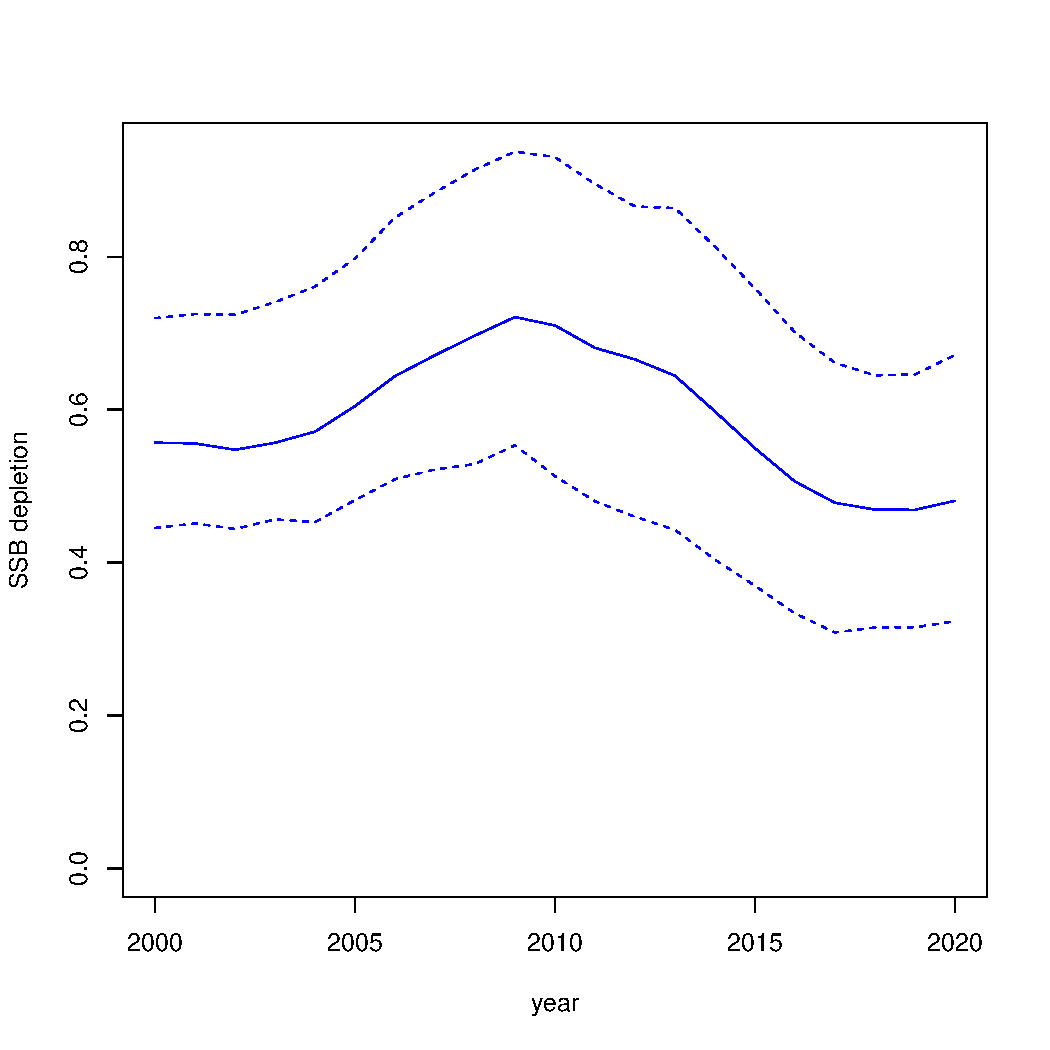
\includegraphics[width=3.5cm,height=3.5cm]{figs/case4a_dep.pdf}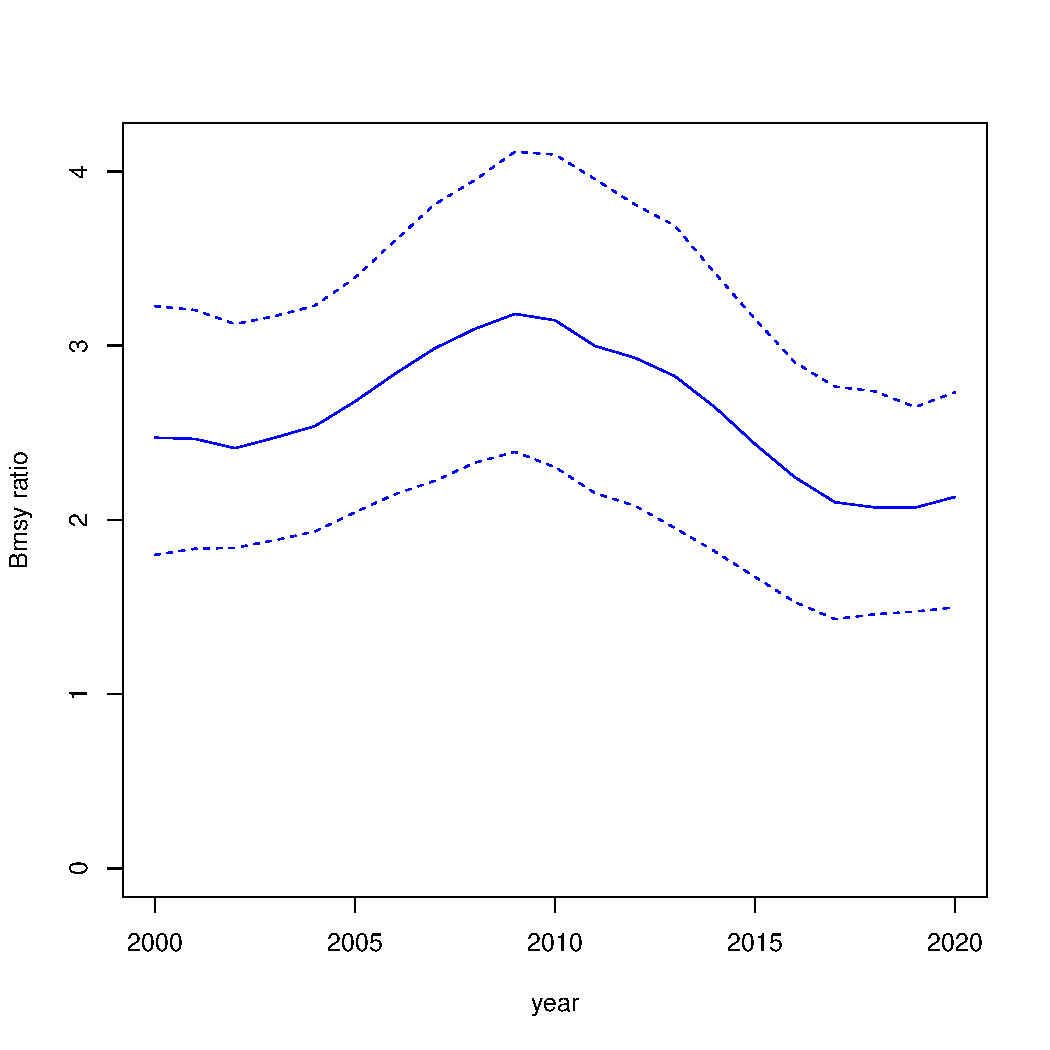
\includegraphics[width=3.5cm,height=3.5cm]{figs/case4a_bmsy.pdf}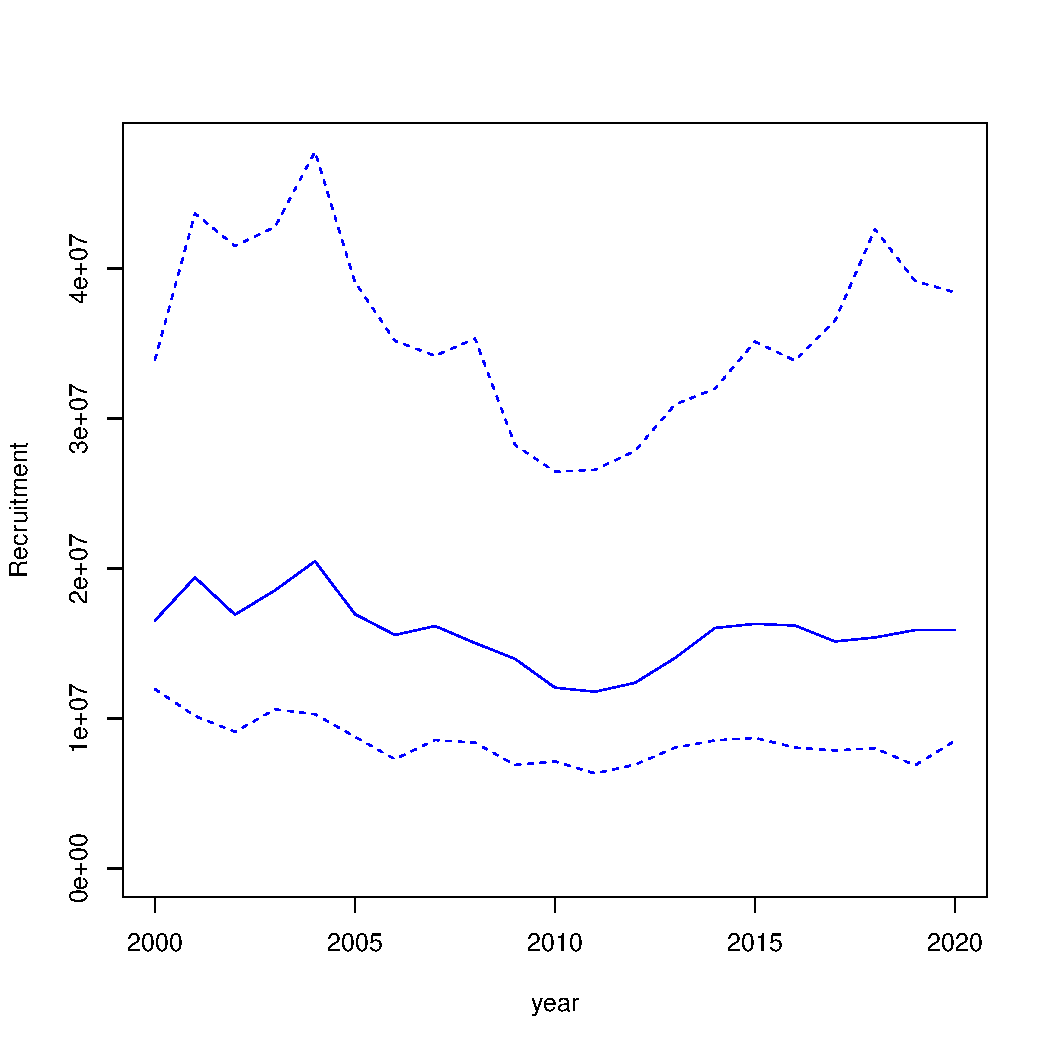
\includegraphics[width=3.5cm,height=3.5cm]{figs/case4a_rec.pdf} 
    \end{center}
\end{figure}
\end{frame}
% frame 14
\begin{frame}
    \frametitle{Selectivity (size-based)}
\begin{itemize}
    \item Scenario \textbf{R1} (top) \& \textbf{R1a} (bottom):
\end{itemize}
\vspace{0.25cm}
\begin{figure}
\begin{center}
       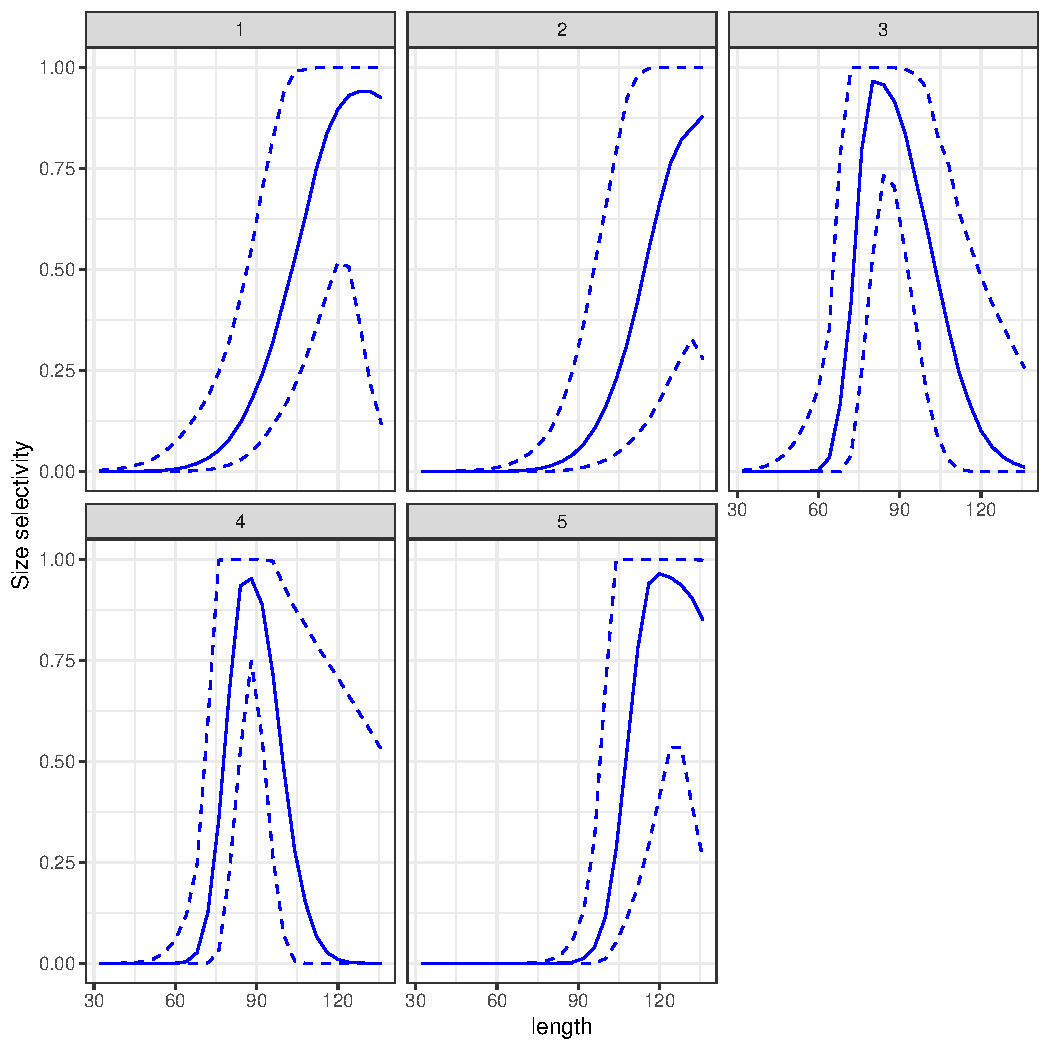
\includegraphics[width=5.5cm,height=5.5cm]{figs/case4_lengthsel.pdf} 
        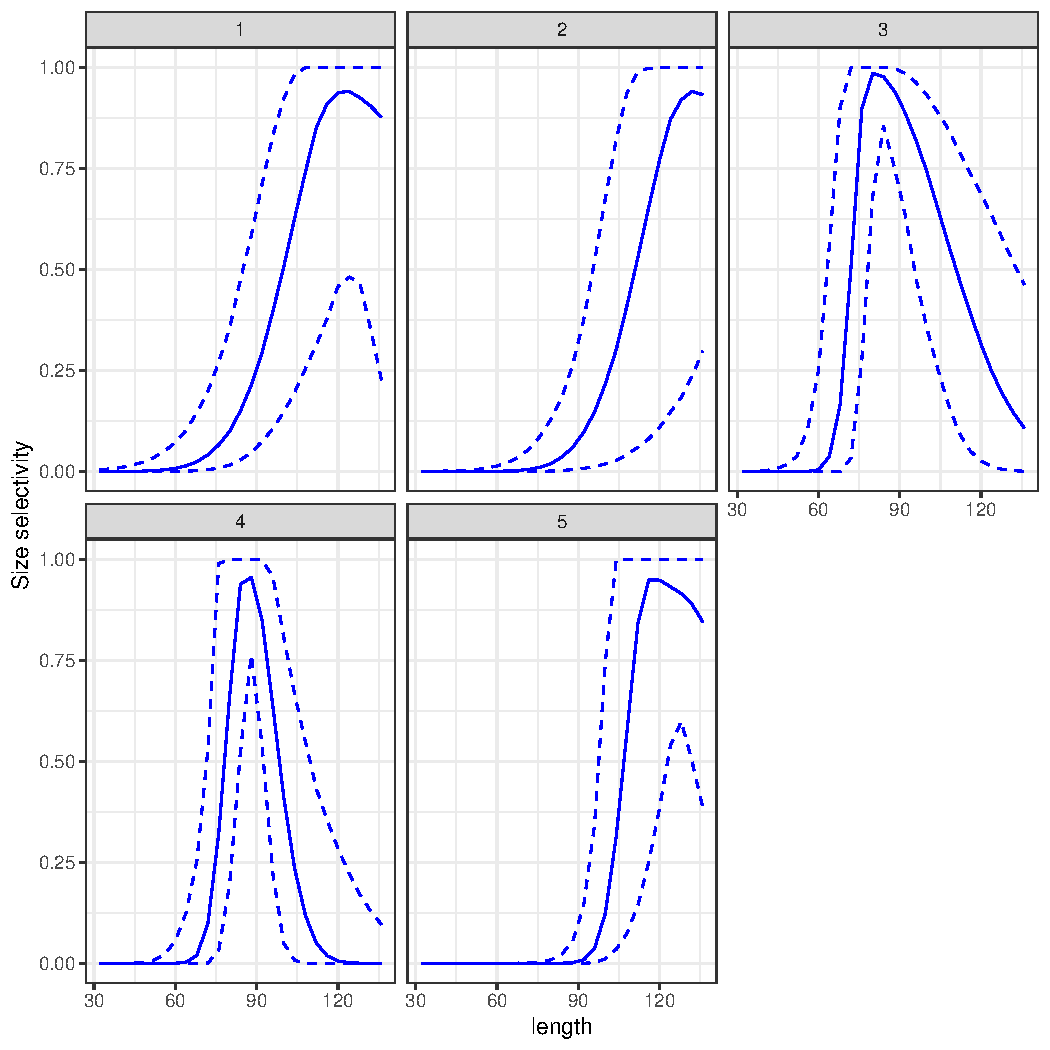
\includegraphics[width=5.5cm,height=5.5cm]{figs/case4a_lengthsel.pdf} 
    \end{center}
\end{figure}
\end{frame}
% frame 15
\begin{frame}
    \frametitle{Estimates of $\sigr$}
\begin{itemize}
    \item Scenario \textbf{R2} (top) \& \textbf{R2a} (bottom):
\end{itemize}
\vspace{0.25cm}
\begin{figure}
\begin{center}
       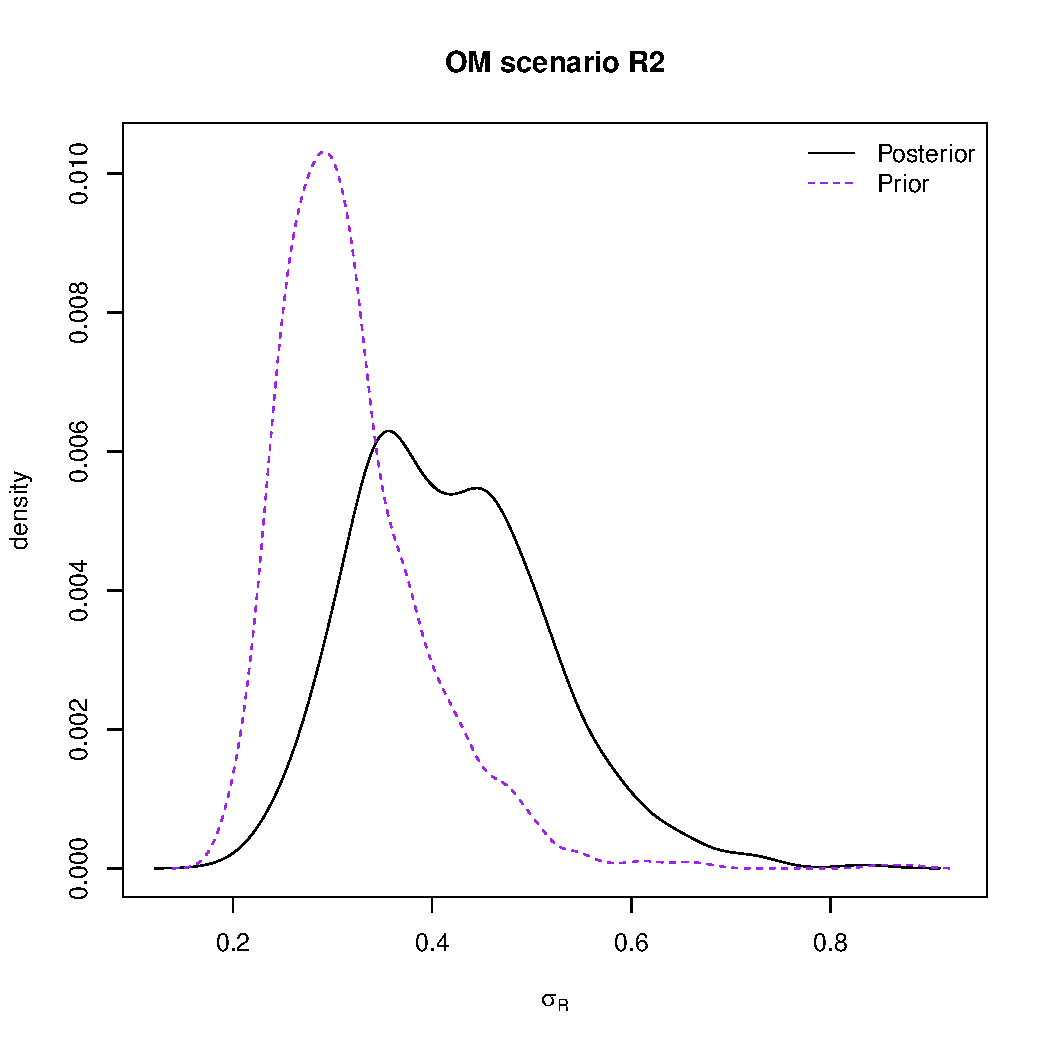
\includegraphics[width=5.5cm,height=5.5cm]{figs/pvsp_sigmar_R2.pdf} 
        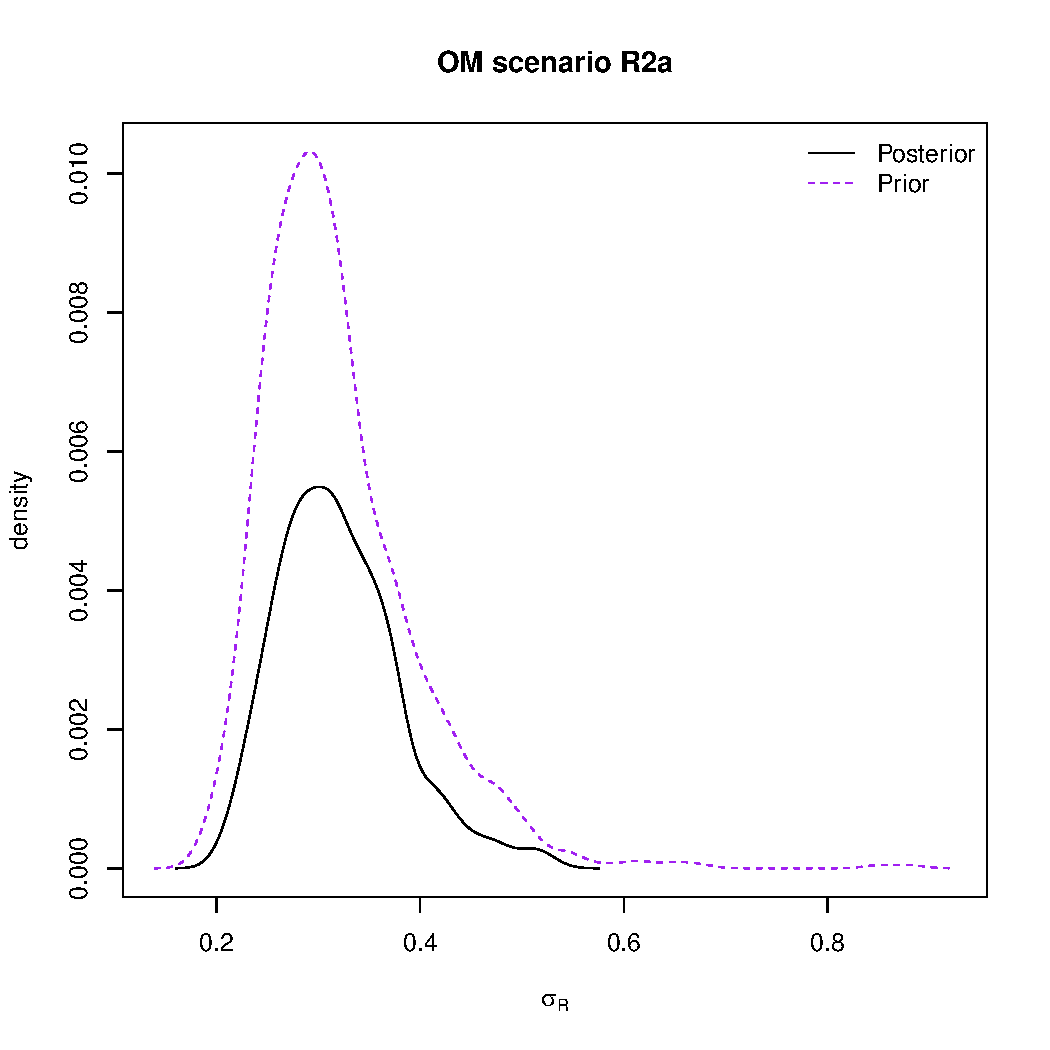
\includegraphics[width=5.5cm,height=5.5cm]{figs/pvsp_sigmar_R2a.pdf} 
    \end{center}
\end{figure}
\end{frame}
% frame 16
\begin{frame}
    \frametitle{OM conditioning summary}
\begin{itemize}
    \item General summary across all OM scenarios:
\end{itemize}
    \tiny{
\begin{table}
    \begin{center}
        \begin{tabular}{|ccccc|}
            \hline
            & & & & \\
            OM scenario & $\Delta_{2000}$ & $\Delta_{2020}$ & $\tdel_{2020}$ & $\mathcal{H}_{2020}$\\
            & & & & \\
Prior & 0.5 (0.3–0.7)    & n/a              & 2 (1.3–2.7)      & 0.6 (0.2–1) \\
R1    & 0.76 (0.61–0.97) & 0.41 (0.22-0.56) & 1.9 (1.02–2.58)  & 1.13 (0.5-3.78) \\
R1a   & 0.56 (0.4–0.72)  & 0.48 (0.3–0.69)  & 2.01 (1.42–2.61) & 0.68 (0.33–1.38) \\
R1b   & 0.74 (0.61–0.9)  & 0.42 (0.24–0.54) & 1.98 (1.16–2.49) & 0.98 (0.46–2.4) \\
R2    & 0.71 (0.57–0.84) & 0.41 (0.21–0.55) & 1.91 (0.99–2.53) & 1.22 (0.45–3.57) \\
R2a   & 0.56 (0.41–0.72) & 0.47 (0.28–0.71) & 2.03 (1.3–2.54)  & 0.65 (0.34–1.4) \\
R2a   & 0.58 (0.40–0.69) & 0.46 (0.28–0.74) & 1.98 (1.35–2.59)  & 0.72 (0.39–1.34) \\
R3    & 0.78 (0.6–0.91)  & 0.38 (0.15–0.52) & 1.77 (0.7–2.44)  & 1.4 (0.58–5.06) \\
R3a   & 0.63 (0.48–0.77) & 0.42 (0.25–0.59) & 1.94 (1.23–2.5)  & 0.71 (0.35–1.45) \\
            & & & & \\
            \hline
        \end{tabular}
    \end{center}
\end{table}
}
\end{frame}
% frame 17
\begin{frame}
    \frametitle{OM conditioning summary}
\begin{itemize}
    \item \textbf{R1}: CPUE inform scale, high upper CI $\mathcal{H}_y$ by 2020
    \item \textbf{R1a}: CPUE uninformative on scale requires $\hmsy$ priors
    \item \textbf{R1b}: \emph{very} similar to \textbf{R1}, removes v. high late $\mathcal{H}_y$
    \item \textbf{R2}: pushes for higher $\sigr$ median 0.41 \vs 0.3
    \item \textbf{R2a}: very consistent with 0.3 - just increases certainty
    \item \textbf{R2b}: potential reference case
    \item \textbf{R3}: similar to \textbf{R1} but more pessimistic recently
    \item \textbf{R3a}: similar to \textbf{R1a} but more pessimistic recently 
\end{itemize}
\end{frame}

% frame 18
\begin{frame}
    \frametitle{Operating model grids}
\begin{itemize}
    \item Reference set: full MCMC samples from OM 2b
    \item Robustness OMs set: 2a, 3
    \item Robustness scenarios: 
        \begin{enumerate} 
            \item future recruitment ``failure'' 
            \item catchability ``regimes''
            \item Trends in growth/maturity/natural mortality
            \item alternative precision scenarios for CPUE
            \item Implementation error alternatives
        \end{enumerate}
\end{itemize}
\end{frame}

% frame 19
\begin{frame}
    \frametitle{Projection dynamics}
\begin{itemize}
    \item Comparing run 2b (L) \& 2a (R) on 30,000 \& 40,000t
\end{itemize}
    \begin{figure}
    \begin{center}   
        \includegraphics[width=4cm,height=4cm]{figs/run5b_dep_proj_40k.pdf}\includegraphics[width=4cm,height=4cm]{figs/run5a_dep_proj_40k.pdf}
        \includegraphics[width=4cm,height=4cm]{figs/run5b_dep_proj_30k.pdf}\includegraphics[width=4cm,height=4cm]{figs/run5a_dep_proj_30k.pdf} 
    \end{center}
    \end{figure}
\end{frame}


% frame 18
\begin{frame}
    \frametitle{Simulation design}
\begin{itemize}
    \item Tuning for 50, 60 and 70$\%$ Kobe green
    \item CPUE-based MP (as SWO)
    \item Surplus production (JABBA) with buffer HCR
\end{itemize}
\end{frame}

% frame 18
\begin{frame}
    \frametitle{Overall summary}
\begin{itemize}
    \item Successful application of ABC OM approach to IO ALB 
    \item Focussed on 2000--2020 time-period (all living cohorts)
    \item Able to fit to all key data sources
    \item Mimics assessment model structure \& status if required
    \item Able to cover previous uncertainty grid probabilistically
    \item Coherent range of plausible OMs
    \item Able to generate key MP data inputs
\end{itemize}
\end{frame}

% frame 19
\begin{frame}
    \frametitle{Next steps: OM}
\begin{itemize}
    \item Implementing Bayesian cross-validation (comp. hard...)
    \item Future work: Possible spatial extensions (conflicting CPUE trends)
\end{itemize}
\end{frame}

% frame 19
\begin{frame}
    \frametitle{Next steps: Which CPUE series?}
\begin{itemize}
    \item \textit{A priori} fleets 1 and 3 plausible
    \item Fleet 1 gives more information on scale
    \item Fleet 3 implies more optimistic current status
    \item MASE for CPUE fleet 1 (L) and 3 (right)
\end{itemize}
    \begin{figure}
    \begin{center}   
        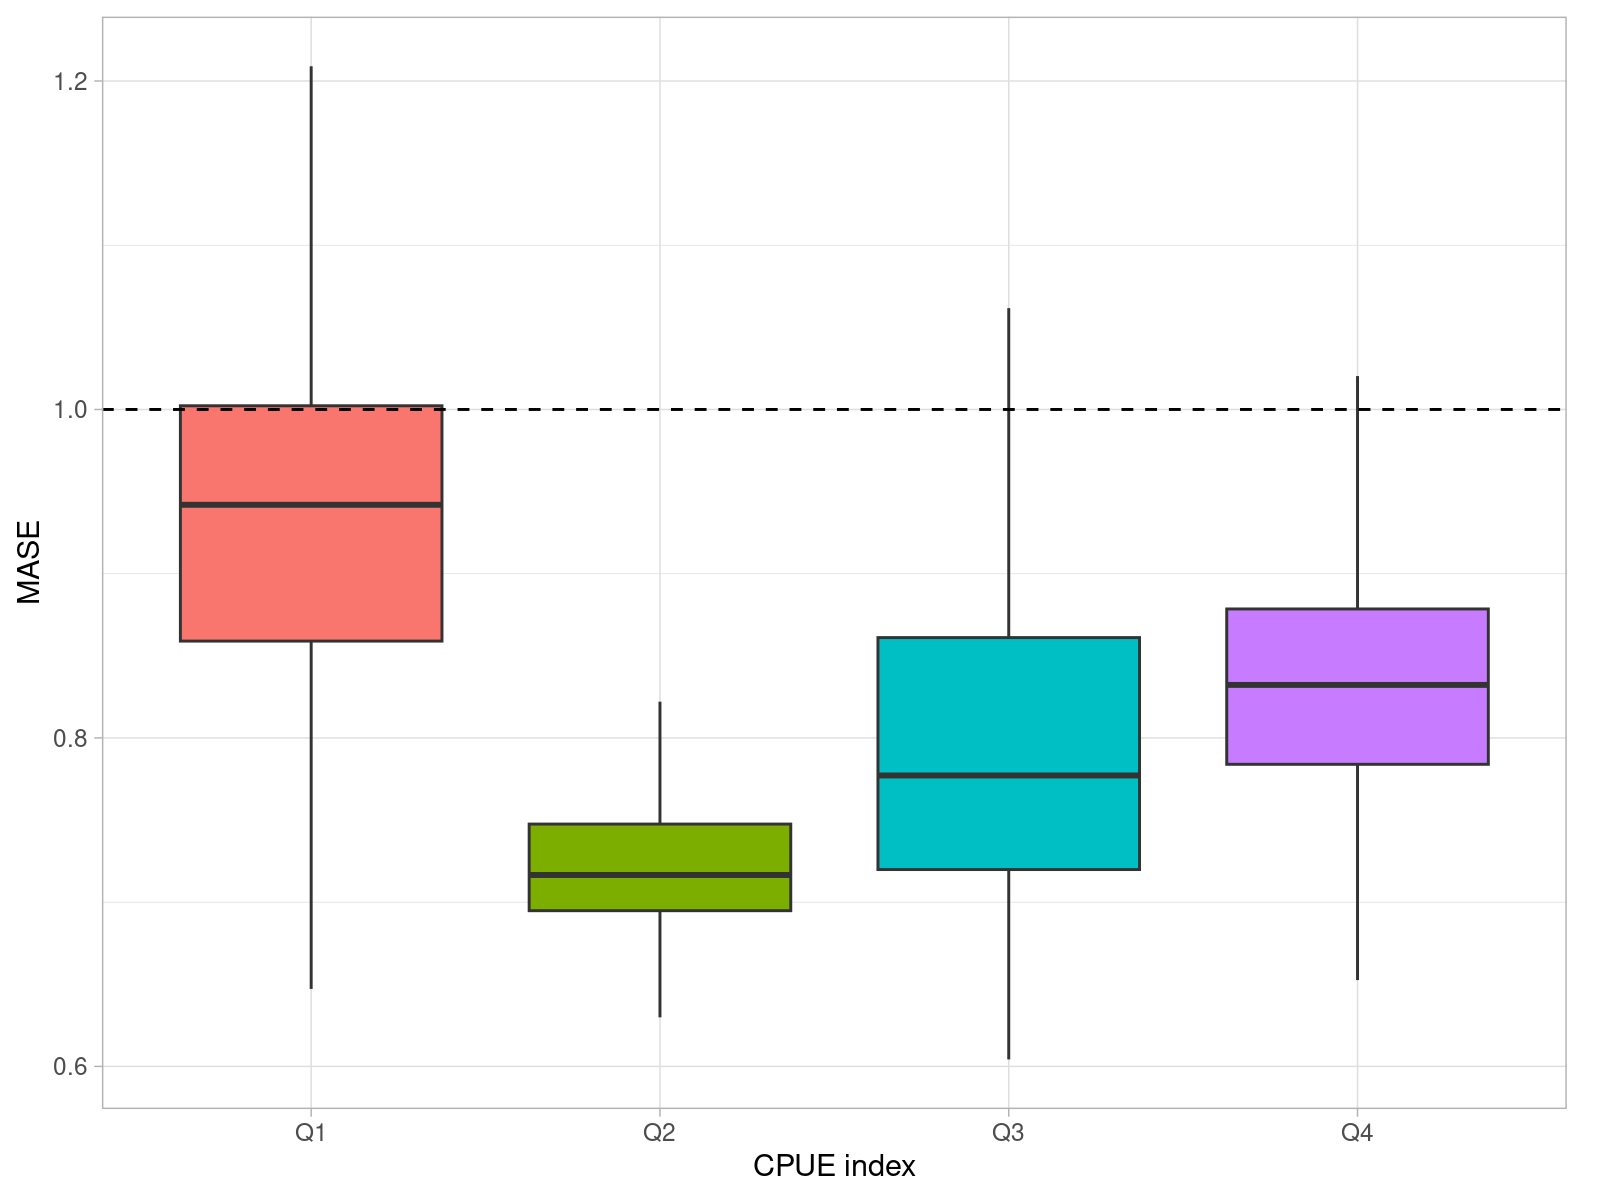
\includegraphics[width=4.5cm,height=4.5cm]{figs/mase/r5bmase.png}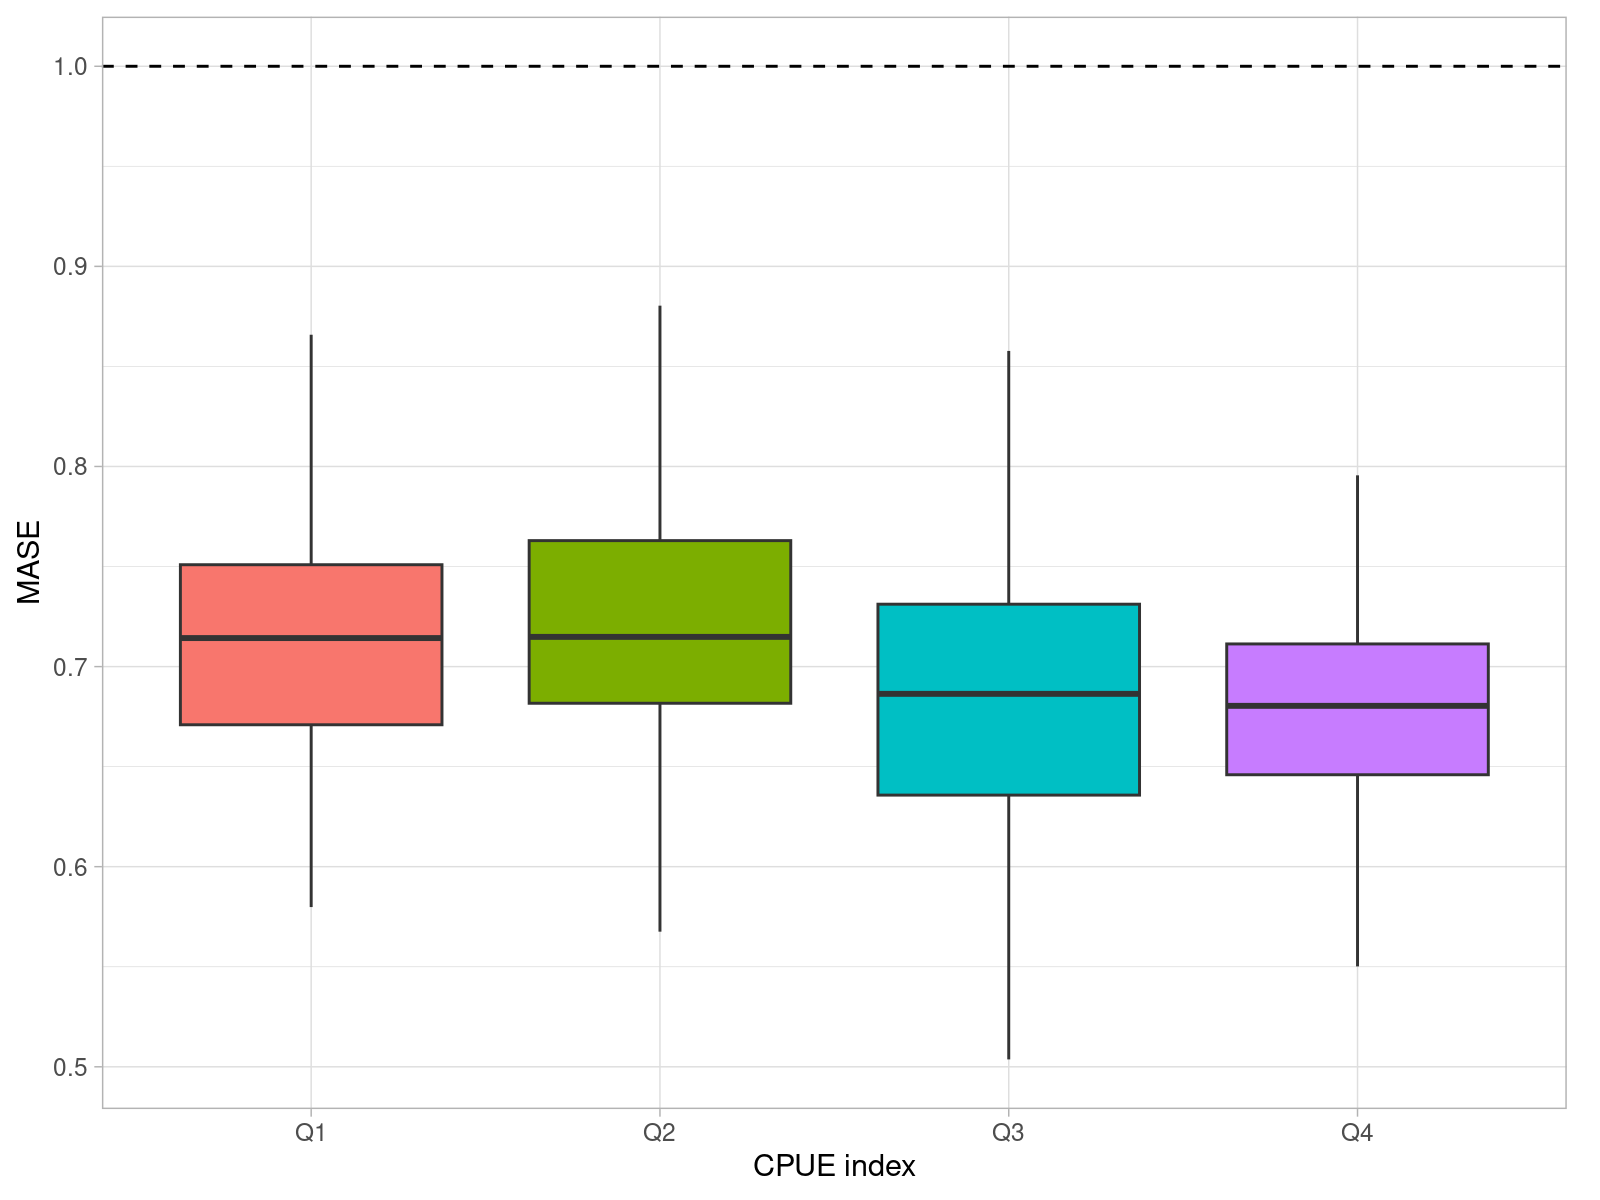
\includegraphics[width=4.5cm,height=4.5cm]{figs/mase/r5amase.png}
    \end{center}
    \end{figure}
\end{frame}

% frame 19
\begin{frame}
    \frametitle{Next steps: MPs}
\begin{itemize}
    \item Testing model-free and JABBA-based MPs
    \item Tuning for all three objectives
    \item Robustness tests
\end{itemize}
\end{frame}

% frame 19
\begin{frame}
    \frametitle{Thanks}
\begin{itemize}
    \item Happy to take comments/questions
\end{itemize}
\end{frame}

%%%%%%%%%%%%%%%%%%%%%%%%%%%%%%%%%%%%%%%%%%%%%%%%%%%
\end{document}
